\documentclass{article}
\usepackage[a4paper,width=150mm,top=25mm,bottom=25mm]{geometry}
\usepackage[utf8]{inputenc}

%%%% Standard Packages
\usepackage{lineno}
\usepackage[hidelinks]{hyperref} 
\usepackage{amsmath}
\usepackage{amssymb}
\usepackage{amsthm}
\usepackage{svg}
\usepackage{cleveref}
\usepackage[fleqn,tbtags]{mathtools}
\usepackage{amsfonts}
\usepackage{standalone}
\usepackage{environ}
\usepackage{slashed}
\usepackage{textcomp}
%\usepackage{subfig}
\usepackage{subfigure}
\usepackage{soul}
\usepackage{xstring}
\usepackage{siunitx}
\usepackage{glossaries}
\makeglossaries
\usepackage{Lib-Notation} %% User define package 


\title{Hermitian quadrature of Gaussian-weighted functions for (proudly) low-tech people}
\author{Miguel Molinos}
\date{September 2022}

\begin{document}

\maketitle

\tableofcontents

\section{Motivation}
\label{sec:Motivation}

We recall from (\ref{eq:ESM:av}) that
\begin{equation}
    \langle V \rangle_0
    =
    \sum_{\{{n}\}\in\mathcal{O}_{NM}} \frac{1}{h^{3N}}
    \int_{\Gamma}
    V(\{{q}\}, \{{n}\})
    \;
    \rho_0(\{{q}\}, \{{p}\}, \{{n}\})
    \, dq \, dp ,
\end{equation}
which in view of (\ref{eq:trialP_MH}) reduces to
\begin{equation}
\label{eq:mean-field-potential-jensen}
    \langle V \rangle_0
    =
    \sum_{\{{n}\}\in\mathcal{O}_{NM}}
    \int
        V_i(\{{q}\}, \{{n}\})
        \Bigg(
            \prod_{j\in{I_\text{M} \cup I_\text{H}}}
            \frac{1}{(\sqrt{2\pi}\sigma_j)^3}
            \exp
            \Big(
                -
                \frac{1}{2\bar{\sigma}_j^2}|{q}_j - \bar{{q}}_j|^2
            \Big)
        \Bigg)
        \Bigg(
            \prod_{j\in I_\text{H}}
            \frac
            {
                {\rm e}^{(\bar{\gamma}_{j}+\gamma_j) n_i}
            }
            {
                1 + {\rm e}^{\bar{\gamma}_{i}+\gamma_i}
            }
        \Bigg)
    \, dq .
\end{equation}
We resort to two approximations to evaluate the requisite phase average. In order to avoid occupancy sums of combinatorial complexity, we apply Jensen's inequality as an equality, with the result
\begin{equation}
    \langle V \rangle_0
    \approx
    \int
        V(\{{q}\}, \{{x}\})
        \Bigg(
            \prod_{j\in{I_\text{M} \cup I_\text{H}}}
            \frac{1}{(\sqrt{2\pi}\sigma_j)^3}
            \exp
            \Big(
                -
                \frac{1}{2\bar{\sigma}_j^2}|{q}_j - \bar{{q}}_j|^2
            \Big)
        \Bigg)
    \, dq .
\end{equation}
In view of the Gaussian weights, we further approximate the integral by Hermitian quadrature, eq.~(\ref{Approximation}), with the result,
\begin{subequations}
\begin{align}
    &
    \langle V \rangle_0
    \approx
    \sum_{k=1}^M V(\{{q}\}_k, \{{x}\}) \, W_k ,
    \\ &
    \langle \frac{\partial V}{\partial q_i} \rangle_0
    \approx
    \sum_{k=1}^M \frac{\partial V}{\partial q_i} (\{{q}\}_k, \{{x}\}) \, W_k ,
\end{align}
\end{subequations}
{\sl et cetera}, where $\{{q}\}_k$ and $W_k$ are $3N$-dimensional Hermitian quadrature points and weights, respectively, centered at $\{\bar{q}\}$ and scaled by $\{\bar{\sigma}\}$.

\section{Numerical quadrature}
\label{sec:Numerical quadrature}

We present a brief summary of the third and fifth degree quadrature rules for multiple integrals in a space of dimension $n$ used in our calculations. The expressions and the quadrature tables were obtained from the work of A. H. Stroud \cite{stroud1971approximate}. In particular, we are interested in the following integrals with gaussian weighting functions:
\begin{equation}\label{Integral}
    I(f)
    =
    \int_{-\infty}^\infty
    \cdots
    \int_{-\infty}^\infty
    f(x_1,\dots,x_n)
    \,\exp[-x_1^2 - \cdots - x_n^2]
    \, dx_1\dots dx_n .
\end{equation}
An $M$-point numerical quadrature approximates the integral as
\begin{equation}\label{Approximation}
    I(f) \approx \sum_{k=1}^M f(\nu_k)W_k \,,
\end{equation}
where $\nu_k$ is an $n$-dimensional vector at the $k^{th}$ quadrature point
\begin{equation}
    \mathbf{\nu}_k = {\nu_{1k},\ldots, \nu_{nk}} \,.
\end{equation}
The expressions for the quadrature points and the associated weights are given below.

\paragraph{Third-degree quadrature} This formula has $2n$ points. The points and coefficients are obtained by requiring that the formula should integrate all monomials of degree $\leq 3$ exactly. Since the domain of integration is $\mathbb{R}^n$ and the Gaussian weight has the property
\begin{equation}
\label{eq:gauss-function-symmetry}
    w(x) = w(-x) \,,
\end{equation}
the distribution of quadrature points is assumed to be fully symmetric. That is, we assume that the formula consists of $2n$ points $\nu_k$ and $-\nu_k$ and that the coefficient of $\nu_k$ equals that of $-\nu_k$. Thus, for an $n$-dimensional space, the points are
\begin{subequations}
\begin{align}
    & (\pm\, r,0, \ldots, 0) \nonumber\\
    & \vdots \nonumber \\
    & (0,\ldots, 0, \pm\, r) \nonumber
\end{align}
\end{subequations}
with the coefficient
\begin{equation}
    W_k = \frac{1}{2n}V,\,\,\, k = 1, \ldots, n \,,
\end{equation}
where
\begin{equation}
    V = I(1) = \pi^{n/2},\,\,\,r^2 = \frac{n}{2}\,.
\end{equation}

\paragraph{Fifth-degree quadrature} This formula has $n^2 + n + 2$ points. The formula is obtained by requiring that it be exact for all monomials of degree $\leq 5$. Owing to the symmetry of the domain, the formula consists of $\frac{1}{2}(n^2 + n +2)$ points $\nu_k$ and their negatives, $-\nu_k$. The coefficient of $\nu_k$ equals that of $-\nu_k$. For an $n$-dimensional space, the $5^{th}$ degree quadrature points and their coefficients can be written as follows using 8 parameters:
\begin{equation}
\begin{split}
    & (\eta, \eta, \ldots, \eta, \eta) \,\,\,\, A \\
    & (\lambda, \xi, \ldots, \xi, \xi) \,\,\,\, B  \\
    & \vdots \\
    & (\xi, \xi, \ldots, \xi, \lambda) \,\,\,\, B  \\
    & (\mu, \mu, \gamma, \ldots, \gamma) \,\,\,\, C  \\
    & (\mu, \gamma, \mu, \ldots, \gamma) \,\,\,\,C  \\
    & \vdots \nonumber \\
    & (\gamma, \ldots, \gamma, \mu, \mu) \,\,\,\, C \\
    & (-\eta, -\eta, \ldots, -\eta, -\eta) \,\,\,\, A  \\
    & (-\lambda, -\xi, \ldots, -\xi, -\xi) \,\,\,\, B \\
    & \vdots \\
    & (-\xi, -\xi, \ldots, -\xi, -\lambda) \,\,\,\, B  \\
    & (-\mu, -\mu, -\gamma, \ldots, -\gamma) \,\,\,\, C  \\
    & (-\mu, -\gamma, -\mu, \ldots, -\gamma) \,\,\,\, C  \\
    & \vdots \\
    & (-\gamma, \ldots, -\gamma, -\mu, -\mu) \,\,\,\, C\,.
\end{split}
\end{equation}
The values of the eight parameters for different dimensions are provided in \cite{stroud1966some,stroud1967some}.

\section{Variable change}
\label{sec:Variable change}

In this section we aim to solve integrals with gaussian weighs of the type:

\subsection{Function type: $h(q_1 , \ldots , q_N)\ s.t\ q_i \in \mathbb{R}$}

Consider a function $h(q_1 , \ldots , q_N)\ s.t\ q_i \in \mathbb{R}$ defined in the range $(-\infty , \infty)$, where each $q_i$ is normally distributed, {\it i.e} $q_i \sim \mathcal{N}(\overline{q}_i , \overline{\sigma}_i^{2})$. The expectation, or mean value, of h corresponds to the following integral:

\begin{equation}
\label{eq:mean-1}
    \langle h \rangle\ =\ \int^{\infty}_{-\infty}\ h(q_1 , \ldots , q_N)\ \prod_{j}^{N}\frac{1}{\overline{\sigma}_j\sqrt{2\pi}} \text{exp}\left(- \frac{(q_j - \overline{q}_j)^2}{2 \overline{\sigma}_j^2}\right)\ dV_q.
\end{equation}

As we can see \cref{eq:mean-1} does not exactly correspond to the Hermite polynomial. To overcome this limitation the following variable change is applied:

\begin{equation}
\label{eq:variable-change-1}
   q_i\ =\ \overline{q}_i\ +\ \overline{\sigma}_i\sqrt{2}\zeta_i\ \quad \rightarrow\ \quad \frac{q_i - \overline{q}_i}{\overline{\sigma}_i\sqrt{2}}\ =\ \zeta_i
\end{equation}

Due to the variable change it is necessary to modify the integration domain. This require the derivation of the corresponding Jacobian for the transformation:

\begin{equation}
\label{eq:jacobian-1}
    dV_q\ =\ \prod_{i}^{N} dq_i\ =\ \prod_{i}^{N} \sqrt{2}\overline{\sigma}_i d\zeta_i\ =\ \prod_{i}^{N} \frac{d q_i}{d \zeta_i}\ dV_{\zeta} =\ \prod_{i}^{N} \sqrt{2}\overline{\sigma}_i\ dV_{\zeta}\
\end{equation}

Introducing \cref{eq:jacobian-1} into \cref{eq:mean-1}:

\begin{equation}
    \begin{split}
        \langle h \rangle\ &=\ \int^{\infty}_{-\infty}\ h(q_1,\ \ldots,\ q_N)\ \prod_{j}^{N}\ \frac{1}{\overline{\sigma}_j\sqrt{2\pi}} \text{exp}\left(- \frac{(\overline{q}_j + \zeta_j \sqrt{2}\overline{\sigma}_j - \overline{q}_j)^2}{2 \overline{\sigma}_j^2}\right)\ dV_q \\
        &=\ \int^{\infty}_{-\infty}\ h(\overline{q}_1\ +\ \overline{\sigma}_1\sqrt{2}\zeta_1,\ \ldots,\, \overline{q}_N\ +\ \overline{\sigma}_N\sqrt{2}\zeta_N)\ \prod_{j}^{N}\ \frac{1}{\overline{\sigma}_j\sqrt{2\pi}} \text{exp}\left(- \zeta_j^2 \right)\  \prod_{j}^{N} \sqrt{2}\overline{\sigma}_j\ dV_{\zeta} \\
        &=\ \int^{\infty}_{-\infty}\ h(\overline{q}_1\ +\ \overline{\sigma}_1\sqrt{2}\zeta_1,\ \ldots,\ \overline{q}_N\ +\ \overline{\sigma}_N\sqrt{2}\zeta_N)\ \prod_{j}^{N}\ \frac{1}{\sqrt{\pi}} \text{exp}\left(- \zeta_j^2\right)\ dV_{\zeta} \\ 
        &=\ \int^{\infty}_{-\infty}\ h(\zeta_1,\ \ldots,\ \zeta_N)\ \prod_{j}^{N}\ \frac{1}{\sqrt{\pi}} \text{exp}\left(- \zeta_j^2\right)\ dV_{\zeta} \\
        &=\ \frac{1}{\pi^{N/2}} \int^{\infty}_{-\infty}\ h(\zeta_1,\ \ldots,\ \zeta_N)\  \prod_{j}^{N} \text{exp}\left(- \zeta_j^2\right)\ dV_{\zeta}
    \end{split}
\end{equation}

Finally the integral is solved numerically simply by evaluation of this expression:

\begin{equation}
\langle h \rangle\ =\ \frac{1}{\pi^{N/2}} \int^{\infty}_{-\infty}\ h(\zeta_1,\ \ldots,\ \zeta_N)\  \prod_{j}^{N} \text{exp}\left(- \zeta_j^2\right)\ dV_{\zeta}\ \approx\ \frac{1}{\pi^{N/2}} \sum_{k=1}^M h(\zeta_k)W_k
\end{equation}


\subsection{Function type: $h(\mathbf{q})\ s.t\ \mathbf{q} \in \mathbb{R}^n$}

Consider a function $h(\mathbf{q})\ s.t\ \mathbf{q} \in \mathbb{R}^n$ defined in the range $(-\infty , \infty)$, where $\mathbf{q} = \{q_1, \ldots, q_n \} = \{q_\alpha\}_{\alpha = 1}^{n}$ is a n-dimensional variable normally distributed, {\it i.e} $\mathbf{q} \sim \mathcal{N}(\overline{q} , \overline{\sigma}^{2})$. The expectation, or mean value, of h corresponds to the following integral:

\begin{equation}
\label{eq:mean-2}
    \langle h \rangle\ =\ \int^{\infty}_{-\infty}\ h(\mathbf{q})\ \prod_{\alpha = 1}^{n}\frac{1}{\overline{\sigma}\sqrt{2\pi}} \text{exp}\left(- \frac{(q_\alpha - \overline{q}_\alpha)^2}{2 \overline{\sigma}^2}\right)\ dV_q
\end{equation}

As we can see \cref{eq:mean-2} does not exactly correspond to the Hermite polynomial. To overcome this limitation the following variable change is applied:

\begin{equation}
\label{eq:variable-change-2}
   q_{\alpha}\ =\ \overline{q}_{\alpha}\ +\ \overline{\sigma}\sqrt{2}\zeta_{\alpha},\ \alpha \in (1,n) \quad \rightarrow\ \quad \frac{q_{\alpha} - \overline{q}_{\alpha}}{\overline{\sigma}\sqrt{2}}\ =\ \zeta_{\alpha}
\end{equation}

Notice how symmetry of the gaussian weight enunciated in \cref{eq:gauss-function-symmetry} has been applied in the variable change. Accordingly, it is necessary to modify the integration domain. This require the derivation of the corresponding Jacobian for the transformation:

\begin{equation}
\label{eq:jacobian-2}
    dV_q\ =\ \prod_{\alpha = 1}^{n} dq_{\alpha}\ =\ \prod_{\alpha = 1}^{n} \frac{d q_{\alpha}}{d \zeta_{\alpha}}\ d\zeta_{\alpha}\ =\ \prod_{\alpha = 1}^{n} \sqrt{2}\overline{\sigma}\ d\zeta_{\alpha}\ =\ \left( \sqrt{2}\overline{\sigma} \right)^n\ dV_{\zeta}\
\end{equation}

Introducing \cref{eq:jacobian-2} into \cref{eq:mean-2}:

\begin{equation}
    \begin{split}
        \langle h \rangle\ &=\ \int^{\infty}_{-\infty}\ h(q_1, \ldots, q_n)\ \prod_{\alpha = 1}^{n}\ \frac{1}{\overline{\sigma}\sqrt{2\pi}} \text{exp}\left(- \frac{(\overline{q}_{\alpha} + \zeta_{\alpha} \sqrt{2}\overline{\sigma} - \overline{q}_{\alpha})^2}{2 \overline{\sigma}^2}\right)\ dV_q \\
        &=\ \int^{\infty}_{-\infty}\ h(\overline{q}_1\ +\ \overline{\sigma}\sqrt{2}\zeta_1,\ \ldots,\, \overline{q}_n\ +\ \overline{\sigma}\sqrt{2}\zeta_n)\ \prod_{\alpha}^{n}\ \frac{1}{\overline{\sigma}\sqrt{2\pi}} \text{exp}\left(- \zeta_{\alpha}^2 \right)\  \prod_{\alpha}^{n} \sqrt{2}\overline{\sigma}\ dV_{\zeta} \\
        &=\ \int^{\infty}_{-\infty}\ h(\overline{q}_1\ +\ \overline{\sigma}\sqrt{2}\zeta_1,\ \ldots,\ \overline{q}_n\ +\ \overline{\sigma}\sqrt{2}\zeta_n)\ \prod_{\alpha}^{n}\ \frac{1}{\sqrt{\pi}} \text{exp}\left(- \zeta_{\alpha}^2\right)\ dV_{\zeta} \\ 
        &=\ \int^{\infty}_{-\infty}\ h(\zeta_1,\ \ldots,\ \zeta_n)\ \prod_{\alpha}^{n}\ \frac{1}{\sqrt{\pi}} \text{exp}\left(- \zeta_{\alpha}^2\right)\ dV_{\zeta} \\
        &=\ \frac{1}{\pi^{n/2}} \int^{\infty}_{-\infty}\ h(\zeta)\ \text{exp}\left(- \| \zeta\|^2\right)\ dV_{\zeta}          
    \end{split}
\end{equation}

Finally the integral is evaluated numerically as:

\begin{equation}
\langle h \rangle\ =\ \frac{1}{\pi^{n/2}} \int^{\infty}_{-\infty}\ h(\zeta)\ \text{exp}\left(- \| \zeta\|^2\right)\ dV_{\zeta}\ \approx\ \frac{1}{\pi^{n/2}} \sum_{k=1}^M h(\zeta_k)W_k
\end{equation}


\subsection{Function type: $h(\mathbf{q}_1 , \ldots , \mathbf{q}_N)\ s.t\ \mathbf{q}_i \in  \mathbb{R}^n$}

Consider a function $h(\mathbf{q}_1 , \ldots , \mathbf{q}_N)\ s.t\ \mathbf{q}_i \in \mathbb{R}^n$ defined in the range $(-\infty , \infty)$, where $\mathbf{q}_i = \{q_{i,1}, \ldots, q_{i,n} \} = \{q_{i,\alpha}\}_{\alpha = 1}^{n}$ is set of n-dimensional variables normally distributed, {\it i.e} $\mathbf{q}_i \sim \mathcal{N}(\overline{q}_i , \overline{\sigma}_i^{2})$. The expectation, or mean value, of h corresponds to the following integral:

\begin{equation}
\label{eq:mean-3}
    \langle h \rangle\ =\ \int^{\infty}_{-\infty}\ h(\mathbf{q}_1 , \ldots , \mathbf{q}_N)\ \prod_{j}^{N}\frac{1}{(\overline{\sigma}_j\sqrt{2\pi})^n} \text{exp}\left(- \frac{\| \mathbf{q}_j - \overline{\mathbf{q}}_j \|^2}{2 \overline{\sigma}_j^2}\right)\ dV_q.
\end{equation}

As we can see \cref{eq:mean-3} does not exactly correspond to the Hermite polynomial. To overcome this limitation the following variable change is applied:

\begin{equation}
\label{eq:variable-change-3}
   q_{i,\alpha}\ =\ \overline{q}_{i,\alpha}\ +\ \overline{\sigma}_i\sqrt{2}\zeta_{i,\alpha} \quad \text{and} \quad \alpha \in (1,n)\ ;\ i \in (1,N)  \quad \rightarrow\ \quad \frac{q_{i,\alpha} - \overline{q}_{i,\alpha}}{\overline{\sigma_i}\sqrt{2}}\ =\ \zeta_{i,\alpha}
\end{equation}

Notice how symmetry of the gaussian weight enunciated in \cref{eq:gauss-function-symmetry} has been applied in the variable change. Accordingly, it is necessary to modify the integration domain. This require the derivation of the corresponding Jacobian for the transformation:

\begin{equation}
\label{eq:jacobian-3}
    dV_q\ =\ \prod_{i = 1}^{N} d\mathbf{q}_{i}\ =\ \prod_{i = 1}^{N} \prod_{\alpha = 1}^{n} \frac{d q_{i,\alpha}}{d \zeta_{i,\alpha}}\ d\zeta_{i,\alpha}\ =\ \prod_{i = 1}^{N} (\sqrt{2}\overline{\sigma}_i)^n\ d\zeta_{i}\
\end{equation}

Introducing \cref{eq:jacobian-3} into \cref{eq:mean-3}:
\begin{equation}
    \label{eq:gaussian-quadrature-3}
    \begin{split}
    \langle h \rangle\ &=\ \int^{\infty}_{-\infty}\ h(\mathbf{q}_1 , \ldots , \mathbf{q}_N)\ \prod_{j}^{N}\frac{1}{(\overline{\sigma}_j\sqrt{2\pi})^n} \text{exp}\left(- \frac{\| \mathbf{q}_j - \overline{\mathbf{q}}_j \|^2}{2 \overline{\sigma}_j^2}\right)\ dV_q \\
    &=\ \int^{\infty}_{-\infty}\ h(\overline{\mathbf{q}}_1\ +\ \overline{\sigma}_1\sqrt{2}\zeta_1,\ \ldots,\ \overline{\mathbf{q}}_N\ +\ \overline{\sigma}_N\sqrt{2}\zeta_N)\ \prod_{j}^{N}\ \frac{1}{\pi^{n/2}} \text{exp}\left(- \|\zeta_j\|^2\right)\ dV_{\zeta} \\ 
    &=\ \int^{\infty}_{-\infty}\ h(\zeta_1,\ \ldots,\ \zeta_N)\ \prod_{j}^{N}\ \frac{1}{\pi^{n/2}} \text{exp}\left(- \|\zeta_j\|^2\right)\ dV_{\zeta} \\     
    &=\ \frac{1}{\pi^{n N/2}} \int^{\infty}_{-\infty}\ h(\zeta_1,\ \ldots,\ \zeta_N)\ \prod_{j}^{N}\ \text{exp}\left(- \|\zeta_j\|^2\right)\ dV_{\zeta}      
    \end{split}
\end{equation}

Finally the integral is evaluated numerically as:

\begin{equation}
\langle h \rangle\ =\ \frac{1}{\pi^{n N/2}} \int^{\infty}_{-\infty}\ h(\zeta_1,\ \ldots,\ \zeta_N)\ \prod_{j}^{N}\ \text{exp}\left(- \|\zeta_j\|^2\right)\ dV_{\zeta}\ \approx\ \frac{1}{\pi^{n N/2}} \sum_{k=1}^M h(\zeta_k)W_k
\end{equation}

\section{Integration of a two-sites potential}

If we apply the result obtained in \cref{eq:gaussian-quadrature-3} to solve \cref{eq:mean-field-potential-jensen}. The following expression is obtained:

\begin{equation}
\label{eq:mean-field-2-particles-potential}
\begin{split}
    \langle V \rangle_0 &\approx \int^{\infty}_{-\infty}\ V(\{{q}\}, \{{\chi}\}) \Bigg(\prod_{j\in{I_\text{M} \cup  I_\text{H}}} \frac{1}{(\sqrt{2\pi}\sigma_j)^3} \exp \Big(- \frac{1}{2\bar{\sigma}_j^2}|{q}_j - \bar{{q}}_j|^2 \Big) \Bigg)\ dq\\
    &=\ \int^{\infty}_{-\infty}\ V(\{{\overline{\mathbf{q}}\ +\ \overline{\sigma}\sqrt{2}\zeta}\}, \{{\chi}\})\ \prod_{j}^{N}\ \frac{1}{\pi^{n/2}} \text{exp}\left(- \|\zeta_j\|^2\right)\ dV_{\zeta} \\     
    &=\ \frac{1}{\pi^{n N/2}} \int^{\infty}_{-\infty}\ V(\{{\overline{\mathbf{q}}\ +\ \overline{\sigma}\sqrt{2}\zeta}\}, \{{\chi}\})\ \prod_{j}^{N}\ \text{exp}\left(- \|\zeta_j\|^2\right)\ dV_{\zeta} \\ 
    &\approx\ \frac{1}{\pi^{n N/2}} \sum_{k=1}^{nM} V(\{{\overline{\mathbf{q}}\ +\ \overline{\sigma}\sqrt{2}\zeta_k}\}, \{{\chi}\})\ W_k
\end{split}
\end{equation}

For the particular case of a potential defined in two sites ($i$ and $j$) depending on a 3 dimensional variable ($\mathbf{q}$). Therefore, particularizing for a 6-dimensional integration space with $\mathbf{q} \sim \mathcal{N}(\overline{q} , \overline{\sigma}^{2})$, the integration points are:
\begin{subequations}
\begin{align}
    & (\overline{\mathbf{q}}_i\ \pm\ \overline{\sigma}_i\sqrt{2}\zeta\ ,\ \overline{\mathbf{q}}_j) \nonumber\\
    & (\overline{\mathbf{q}}_i\ ,\ \overline{\mathbf{q}}_j\ \pm\ \overline{\sigma}_j\sqrt{2}\zeta)  \nonumber
\end{align}
\end{subequations}
and the quadrature weights are:
\begin{equation}
    W_k\ =\ \frac{1}{2nN}\ V,\ \quad k = 1, \ldots, nN \,,
\end{equation}
where
\begin{equation}
    V\ =\ I(1)\ =\ \pi^{nN/2},\,\,\,\zeta^2 = \frac{nN}{2}\,.
\end{equation}
See \cref{fig:integration-scheme} for a graphical interpretation of the layout of the integration points. After a careful inspection of \cref{eq:mean-field-2-particles-potential}, the following terms of the final expression require a slight modification:
\begin{align}
\label{eq:quadrature-weight-term}
\frac{1}{\pi^{n N/2}} W_k\ &=\ \frac{1}{\pi^{n N/2}} \frac{V}{2nN}\ =\ \frac{1}{\pi^{n N/2}} \frac{\pi^{nN/2}}{2nN}\ =\ \frac{1}{2\ nN}\ =\ \frac{1}{12} \\
\label{eq:quadrature-position-term}
\overline{\sigma}\sqrt{2}\zeta_k\ &=\ \overline{\sigma}\sqrt{2} \sqrt{\frac{nN}{2}}\ =\ \frac{98.2950}{\omega \sqrt{\beta m}} \sqrt{nN}\ \si{\angstrom}\ =\ \frac{98.2950}{\omega \sqrt{\beta m}} \sqrt{6}\ \si{\angstrom}\
\end{align}

Introducing \cref{eq:quadrature-weight-term,eq:quadrature-position-term} in \cref{eq:mean-field-2-particles-potential} the resulting expression to be implemented is:

\begin{align}
  \langle V \rangle_0\ &\approx\ \sum_{k=1}^{nN} \frac{1}{12}\ V(\{{\overline{\mathbf{q}}\ \pm\ \frac{98.2950}{\omega \sqrt{\beta m}} \sqrt{6}}\ \si{\angstrom}\}, \{{\chi}\})\\
  \langle \frac{\partial V}{\partial q_i} \rangle_0\ &\approx\ \sum_{k=1}^{nN} \frac{1}{12}\ \frac{\partial V}{\partial q_i} (\{{\overline{\mathbf{q}}\ \pm\ \frac{98.2950}{\omega \sqrt{\beta m}} \sqrt{6}}\ \si{\angstrom} \}, \{{\chi}\}).
\end{align}

\begin{figure}
    \centering
    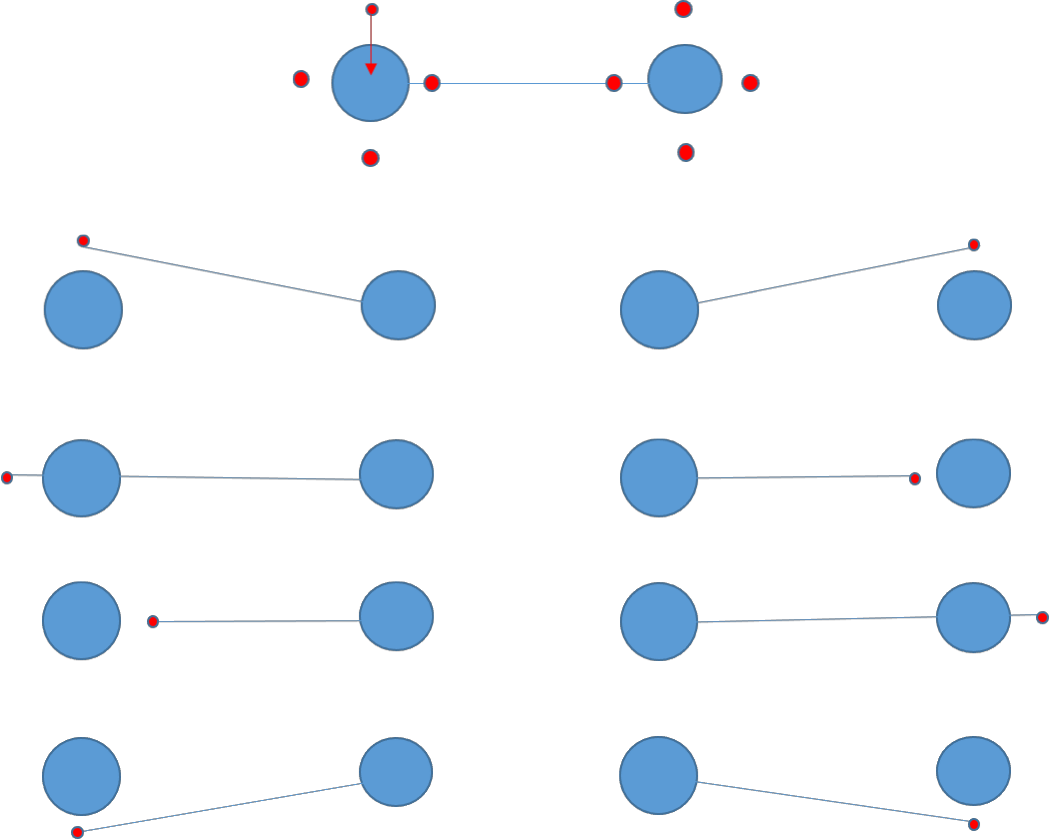
\includegraphics[width=0.8\textwidth]{Integration-points.png}
    \caption{Integration scheme for a two-site potential}
    \label{fig:integration-scheme}
\end{figure}

\bibliographystyle{plain}
\bibliography{biblio}

\end{document}
